\chapter{CubeSat Integration Steps} \label{ch:cubesat-integration-steps}

The CubeSat that will be used in the FloripaSat-2 consists of three modules, OBDH, TTC and EPS, which are the core of the CubeSat, and payloads. In order to facilitate the integrations of all this modules, a testing process had to be created, which will be done using the FlatSat.

This process was divided in five steps, which will be presented in the next sections with more details. First, the core of the CubeSat will be connected together, to evaluate the interaction between them. Then, the GRS will be emulated to verify if there will be no errors in data transmission and reception. Later, all payloads will be connected together with the core of the CubeSat and, later, the GRS will be emulated again. Finally, a long-term evaluation will be made.

\section{CubeSat Core}

In this step, the interaction between OBDH, EPS and TTC will be evaluated. Therefore, the main communication protocols that these three modules use to interact need to be tested. The deployment sequence will be performed with a fully functional EPS and also with a partially functional EPS, to search for critical errors. Subsequently, the operation of these modules will be evaluated.

\subsection{Deployment Sequence}

After the decouple of the satellite, the kill-switches will enable the power supply of the OBDH, EPS and TTC. Actually, the EPS will distribute energy for the EPS and OBDH. After the boot, OBDH waits 45 minutes before operating normally. Then, the OBDH will act to deploy the antennas. Similarly to the ODBH, after de boot, TTC waits 55 minutes before operating normally. Redundantly, the TTC will also act to deploy the antennas. The TTC will enable the sub-modules Downlink/Uplink and Beacon at the end of the process. It repeats indefinitely, but the OBDH and TTC don’t need to wait anymore to operate normally. The figure 6.1 shows the process described.

\begin{figure}[H]
	\begin{center}
		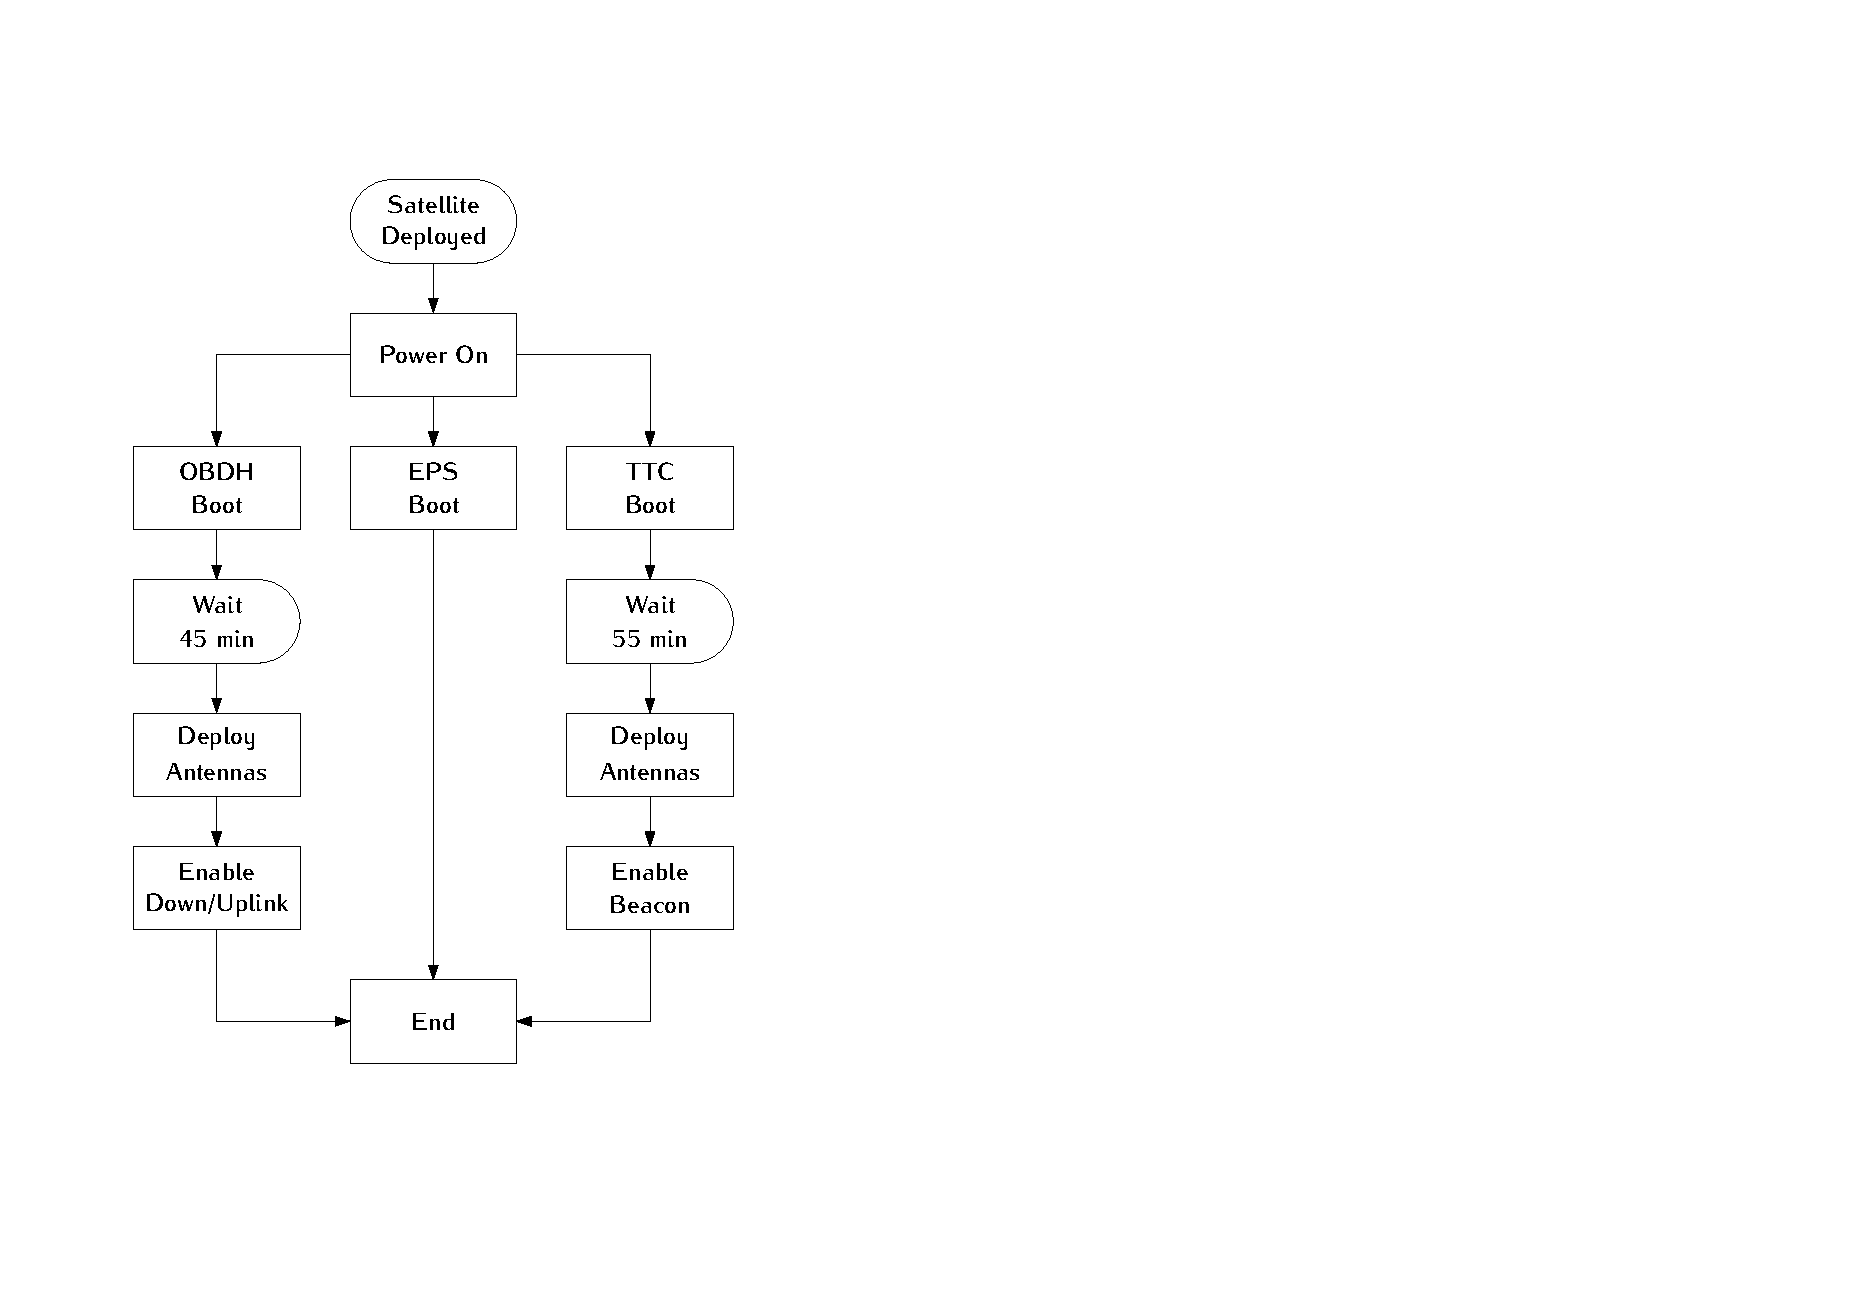
\includegraphics[width=0.5\textwidth]{figures/deployment-flowchart.pdf}
		\caption{Flowchart of the deployment sequence.}
		\label{fig:deployment-flowchart}
	\end{center}
\end{figure}

\subsubsection{Experiment Setup}

First, all three modules will be connected to the FlatSat. The EPS needs to be connected to Slot 1, and the other two modules can be connected in any slots, like in figure 6.2.

\begin{figure}[H]
	\begin{center}
		
\includegraphics[width=0.5\textwidth]{figures/dummy-image.png}
		\caption{OBDH, EPS and TTC connected in the FlatSat.}
		\label{fig:connections-1}
	\end{center}
\end{figure}

Still with the kill-switches cutting-off the power supply for the EPS, a battery is connected to CN10 or CN4. Then, jumpers can used between CN12 or CN6 and the EPS, like in figure 6.3.  

\begin{figure}[H]
	\begin{center}
		
\includegraphics[width=0.5\textwidth]{figures/dummy-image.png}
		\caption{Connecting EPS to an external power supply.}
		\label{fig:connections-1}
	\end{center}
\end{figure}

A launchpad will emulate the antennas, like the MSP-EXP430F5529LP. Then, this launchpad can be connected in the PC-104, so OBDH and TTC can communicate with it, like figure 6.4.

\begin{figure}[H]
	\begin{center}
		
\includegraphics[width=0.5\textwidth]{figures/dummy-image.png}
		\caption{Launchpad emulating the Antenna Module.}
		\label{fig:connections-1}
	\end{center}
\end{figure}

\subsubsection{Waiting Time}

The OBDH and TTC won’t operate normally for 45 minutes and 55 minutes, respectively. The validation criteria for this first experiment is shown in the table 6.1.

\begin{table}[H]
	\centering
	\resizebox{\columnwidth}{!}{\begin{tabular}{cc}
		\toprule[1.5pt]
		\textit{Question} & \textit{Answer} \\
		\midrule
		Is the OBDH doing something before 45 minutes have elapsed?  & No, 45 minutes elapsed before the OBDH act to deploy the antennas. \\
		Is the TTC doing something before 55 minutes have elapsed? & No, 55 minutes elapsed before the TTC act to deploy the antennas. \\
		\bottomrule[1.5pt]
	\end{tabular}}
	\caption{Validation criteria.}
	\label{tab:validation-criteria-1}
\end{table}

\subsubsection{Redudancy}

If OBDH cannot act to deploy the antennas, the TTC needs to act. The validation criteria for this first experiment is shown in the table 6.2.

\begin{table}[H]
	\centering
	\resizebox{\columnwidth}{!}{\begin{tabular}{cc}
			\toprule[1.5pt]
			\textit{Question} & \textit{Answer} \\
			\midrule
			TTC was capable of doing the deployment of the antennas? & Yes, OBDH didn't act and the TTC act correctly.\\
			\bottomrule[1.5pt]
	\end{tabular}}
	\caption{Validation criteria.}
	\label{tab:validation-criteria-2}
\end{table}

\subsubsection{Power Supply}

The EPS uses the MPPT, a method used to distribute energy with more efficiency. But, if the EPS cannot implement this method, theoretically, it would distribute the energy to the other modules, but with less efficiency. But, to guarantee, this need to be evaluated. The validation criteria for this first experiment are shown in the table 6.2.

\begin{table}[H]
	\centering
	\resizebox{\columnwidth}{!}{\begin{tabular}{cc}
			\toprule[1.5pt]
			\textit{Question} & \textit{Answer} \\
			\midrule
			If the EPS fails to implement the MPPT, OBDH and TTC will boot? & Yes, OBDH and TTC booted.\\
			\bottomrule[1.5pt]
	\end{tabular}}
	\caption{Validation criteria.}
	\label{tab:validation-criteria-2}
\end{table}

\subsection{Interactions}

